\section{Materials and Methods}

    This project will use an artificial lateral line to observe the vortex interaction between 2, two dimensional, tandem flapping foils in USNA's Large Re-Circulating Water Tunnel. First, the commercially available pressure sensors at USNA will be evaluated to determine which is optimal for wake observation based on a predefined set of standards. Next, the identified sensor will be built into an artificial lateral line as inspired by \citep{Venturelli2012}. Then, the sensor array's response to a single vortex street will be analyzed by placing it downstream from a single flapping foil, similar to the initial experiments conducted by \citep{Venturelli2012} and \citep{Boschitsch2014}. Finally, the sensor array will be placed downstream from two, tandem foils flapping at various phases. The data collected from this experiment will be analyzed in MATLAB for features that correlate with the phase difference.

\subsection{The Sensor Array} \label{The Sensor Array}
\subsubsection{Pressure Sensor Characterization} \label{Pressure Sensor Characterization}
     
    Before building an artificial lateral line, it will be necessary to identify and characterize the best available pressure sensor. All sensors are influenced by high frequency noise and low frequency bias drift. While filters can be implemented to minimize the effects of noise, the vortex interactions caused by the tandem fins will register as somewhat high-frequency pressure changes to the sensors, so only a high-pass filter will be created and used to mitigate bias drift. The USNA Hydromechanics Laboratory currently possesses several pressure sensors relevant to this work, and the sensors used in \citep{Venturelli2012} and \citep{Chambers2014} are also readily available.
    
    The Hydromechanics Laboratory's available sensors will be tested and evaluated based on their sampling frequency, noise, bias drift, and sensitivity. The most desirable trait will be low noise, as a higher signal to noise ratio will enable more accurate and consistent readings. The sensors' sensitivities are second most important, as they are the second component of the sensors' signal to noise ratios. The sampling frequency is third most important, as a higher frequency will allow the array to sense vortices that are close together. The bias drift is least important, as it can be largely compensated for using a high-pass filter and calibration.
    
    Each sensor will be mounted to a PVC pipe in stationary water and their data will be collected through their respective interfaces. The sensors' outputs will be recorded for multiple trials, each lasting several minutes. The resultant data will provide information on each sensors' bias drift frequency, which can be eliminated using a high-pass filter of the form
    \begin{equation} \label{Eq:High pass filter}
    x_n=\frac{2-aT}{2+aT}x_{n-1}+\frac{2}{2+aT}(y_n+y_{n-1})
    \end{equation} 
    where \(x_n\) and \(x_{n-1}\) are the current and previous output reading, respectively, \(y_n\) and \(y_{n-1}\) are the current and previous input readings, respectively, \(T\) is the sampling period, and \(a\) is the bias drift frequency found for a sensor. The sampling period is related to the sampling frequency by \(T=\frac{1}{f}\). Applying this filter to each trial's data will leave only high frequency noise for each sensor.
    
    The impact of this noise is directly related to the standard deviation in a given sensor's pressure readings over the trial, as the sensors should ideally measure a single value. Sensors with higher standard deviations will show the highest degree of noise, and this will factor into their selection for use in the lateral line.

%\begin{figure}
%\begin{center}
%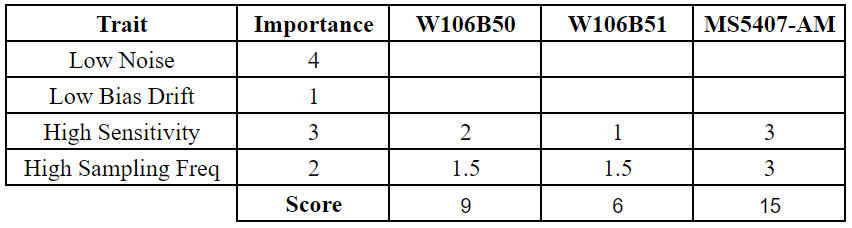
\includegraphics[width=0.8\columnwidth]{figures/Decision Matrix.png}
%\end{center}
%\caption{Decision matrix used to compare the available pressure sensors.}
%\label{fig:methods:Decision Matrix}
%\end{figure}

\subsubsection{Constructing the Sensor Array} \label{Constructing the Sensor Array}
    
    The optimal sensor model identified in Section \ref{Pressure Sensor Characterization} will be built into an artificial lateral line. The sensors will be arranged into two rows inside a PVC tube, positioned on opposite sides of the tube and extending from one end to the other. A cross section of the anticipated layout is shown in \Fref{fig:methods:2D Setup}. The sensors will make contact with the water through pre-drilled holes that are evenly spaced. Their pressure data will be carried through the tube and out its downstream end via coaxial cables. The data will be exported to a laptop computer and analyzed in MATLAB. Several sensors will be used, likely within the range of 8-16 units, depending on the interface required.
    
\subsection{Foil Construction and Actuation} \label{Foil Construction and Actuation}
    
    The foils will be made with a NACA0016 cross section and a chord length, \(C\), of 8 cm. The bodies will be fabricated in the Rickover Model Shop using foam and aluminum. A rod will be placed along the pitch axis, located one quarter chord behind the leading edge. The foil setup will resemble that of \citep{Boschitsch2014}, enabling quick data comparison. The NACA0016 foil will lend itself to better inferences from  data, as its characteristics are well documented and understood. The foils will be 0.40 m tall, spanning the height of the Re-Circulating Water Tunnel. 
    
    The foil movements will be programmed with an Mbed microprocessor, and they will be actuated by servomotors from previous bio-inspired propulsion experiments in the Biomechanics Laboratory. To make this project attainable using USNA equipment, the foils will not undergo heave motions, and will only pitch. This motion will still achieve the necessary vortex interactions that highlight thrust generation as a function of the foils' phase difference. The foil cross sections and a sketch of the 3D setup can be found in \Fref{fig:methods:2D Setup} and \Fref{fig:methods:3D Setup}, respectively. When placed in tandem, the foils will move according to the equations given in \Fref{tab:methods:EOM}.
\begin{center}
\begin{table}
\caption{Equations of Foil Motion}
\label{tab:methods:EOM}
\begin{tabular}{ccc}
\toprule
Motion & Upstream Foil & Downstream Foil \\ 
\midrule
Pitch & \(\theta(t)=\theta _msin(\omega t)\) & \(\theta (t)=\theta _msin(\omega t+\phi)\) \\
\end{tabular}
\end{table}
\begin{figure}
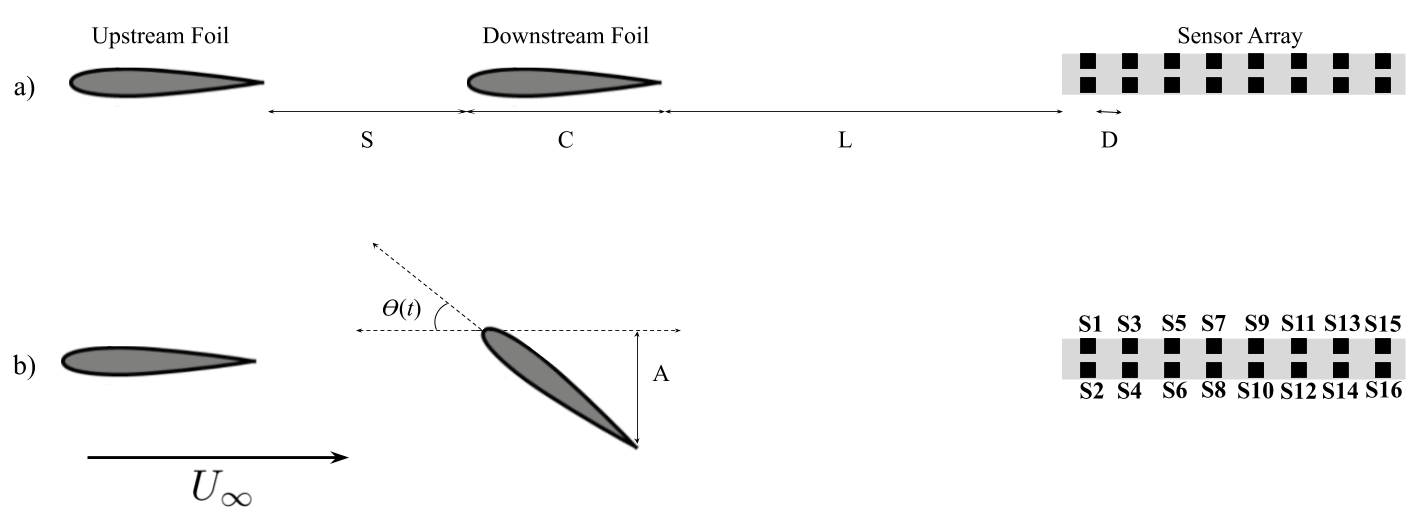
\includegraphics[width=0.8\columnwidth]{figures/Experimental Setup.png}
\caption{Stationary depiction of 2D tandem foil experiment setup with foil spacing, chord length, and sensor spacing marked (a). 2D tandem foils in motion with foil pitch angle, stroke amplitude, and free stream velocity marked (b).}
\label{fig:methods:2D Setup}
\end{figure}
\begin{figure}
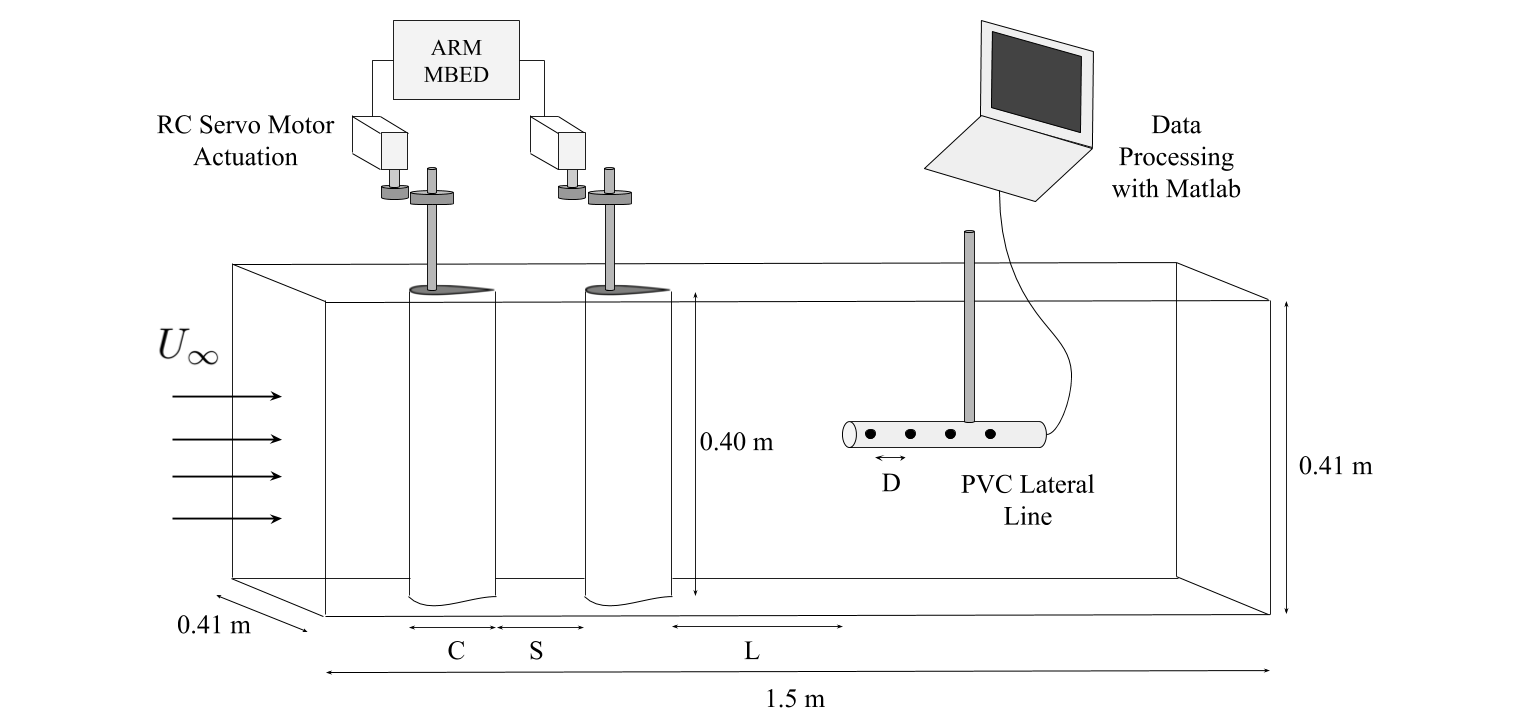
\includegraphics[width=0.95\columnwidth]{figures/3D Tank Setup.png}
\caption{3D depiction of experimental setup with free stream velocity, \(U_\inf\), foil chord, $C$, foil spacing, $S$, distance between the foils and lateral line, $L$, and the spacing of pressure sensors, $D$, marked. The tank dimensions and foil height are also given.}
\label{fig:methods:3D Setup}
\end{figure}
\end{center}

\subsection{Single Foil Test} \label{Single Foil Test}
    
    It will be necessary to study the lateral line's response to a single vortex wake before applying it to tandem foil vortex wakes. This will allow for calibration of sensors and verification of the setup's accuracy, as results can be compared to previous work. This experiment will also determine the best experimental parameters for vortex observation and demonstrate the lateral line's sensitivity to vortex location. In doing so, it will replicate the primary experiments from \citep{Venturelli2012} and \citep{Chambers2014}, as well as the initial test by \citep{Boschitsch2014}. The lateral line constructed in Section \ref{The Sensor Array} will be placed two chord lengths downstream from one foil constructed in Section \ref{Foil Construction and Actuation}, located in the Large Re-Circulating Water Tunnel. This setup is identical to that shown in \Fref{fig:methods:3D Setup}, but the upstream foil is omitted. The trial will begin with the fin at rest for five seconds, the fin will flap for five oscillation cycles, and then it will come to rest for ten seconds. The differential pressure readings between opposite sensors (i.e. s1-s2, s3-s4 in \Fref{fig:methods:2D Setup}) will be collected and analyzed in MATLAB. The average pressure observed during the rest periods will allow for sensor calibration and show if any sensor drift was present during the trial.
    
\subsubsection{Determining Fin Motion Parameters} \label{Determining Fin Motion Parameters}
    
    Several trials will be conducted to determine the optimal fin motion parameters for vortex detection. The fin's Strouhal number will be fixed at 0.25, a relevant value for finned propulsion discussed in Section \ref{Fin Propulsion}. The peak edge displacement, \(A\), free stream velocity, \(U_\inf\), and maximum pitch angle, \(\theta_m\), will be varied until the lateral line's detects the vortices in a similar manner to those in \Fref{fig:PW:Chambers Results}. During this experimentation, the Reynolds number does not need to be matched for an actual fish, as vortex shedding and wake interaction is known to be largely independent of Reynolds number. The motion parameters used in \citep{Boschitsch2014} will provide a starting point for this experimentation. Additionally, this test will help to determine the optimal distance between the foil and lateral line for vortex detection. This value is marked as $L$ in \Fref{fig:methods:2D Setup} and \Fref{fig:methods:3D Setup}.
    
\subsubsection{Testing Lateral Sensitivity} \label{Testing Lateral Sensitivity}
    
    Once the vortex street is consistently perceived, the lateral line will be moved out of the direct path of the vortex wake. This should display characteristics similar to those in \Fref{fig:PW:Chambers Results}, where the sinusoidal vortex signals decreased in amplitude with lateral distance. This step will demonstrate the lateral line's sensitivity to vortex displacement.

\subsection{Tandem Fin Test} \label{Tandem Fin Test}

    After completing baseline tests with a single foil, this project will collect wake data from a tandem foil setup at multiple phase differences. A second foil will be added to the setup described in Section \ref{Single Foil Test}, completing the construction of the sketch in \Fref{fig:methods:3D Setup}. This foil will be positioned upstream of the single foil with a spacing, \(S\), of one chord length, so that the downstream foil will not influence its vortex production \citep{Boschitsch2014, Muscutt2017}. The system will be placed under a constant, uniform flow using the Re-Circulating Water Tunnel's four-bladed axial flow impeller. A series of about twenty-five tests will be conducted where the tandem fins will flap according to the equations given in \Fref{tab:methods:EOM}. Their phase difference, \(\phi\), will differ for each trial and range from 0 to 180°. Each trial will begin with the foils at rest for 5 seconds, the fins will flap for five cycles, and then they will come to rest for ten additional seconds. The pressure readings during the stationary portion of the trial will show the noise and unperturbed water pressure. The constant pressure reading over the last ten seconds will indicate any bias in the pressure readings over the course of the experiment. Three trials will be run for each \(\phi\), yielding a total of seventy-five trials. The differential pressure data will be saved for further analysis described in Section \ref{Data Analysis}.
    
\subsection{Materials}

    The sensors and their interface materials are available through the Hydromechanics Laboratory, while the PVC tubing and its mount are available through the Rickover Model Shop. The foil bodies will be constructed with aluminum and foam in the Model Shop, while the servomotor actuators for the foils will be reused from past independent research projects within the Biomechanics Laboratory. All experiments will take place in the Large Re-Circulating Water Tunnel located in the Hydromechanics Laboratory, whose dimensions are 0.41 m x 0.41 m x 1.50 m.
    
%\subsection{Optional Fluid Simulation}

%    If the experimental procedures and data analysis described above are completed with significant time remaining, an additional objective will be to validate experimental computational fluid dynamics (CFD) models. As described in Section \ref{CFD Attempts}, the Boundary Data Immersion Method (BDIM) has offered a potential route for simulating fluid dynamics in the presence of multiple moving bodies, such as tandem fins. The experimental data developed for this project could be used to validate BDIM-based CFD programs in OpenFoam and Lilypad by running the simulated versions of the trials and comparing the actual and simulated downstream pressures. These CFD methods will take significant time to learn, and this objective will only be pursued if the project is two months ahead of schedule. 